\documentclass{recipe}

\begin{document}
\begin{recipe}{Red Wine, Beef, and Tomato Sauce}
  \servings{2}

  \begin{ingredients}
    \ingredient{1}{tbsp}{butter}
    \ingredient{1}{tbsp}{olive oil}
    \ingredient{8}{oz}{beef chuck steak}
    \ingredient{9}{oz}{Cabernet Sauvignon}
    \ingredient{7.5}{oz}{canned crushed tomatoes}
    \ingredient{10}{oz}{Fettuchini}
  \end{ingredients}

  \begin{images}
    \begin{image}
      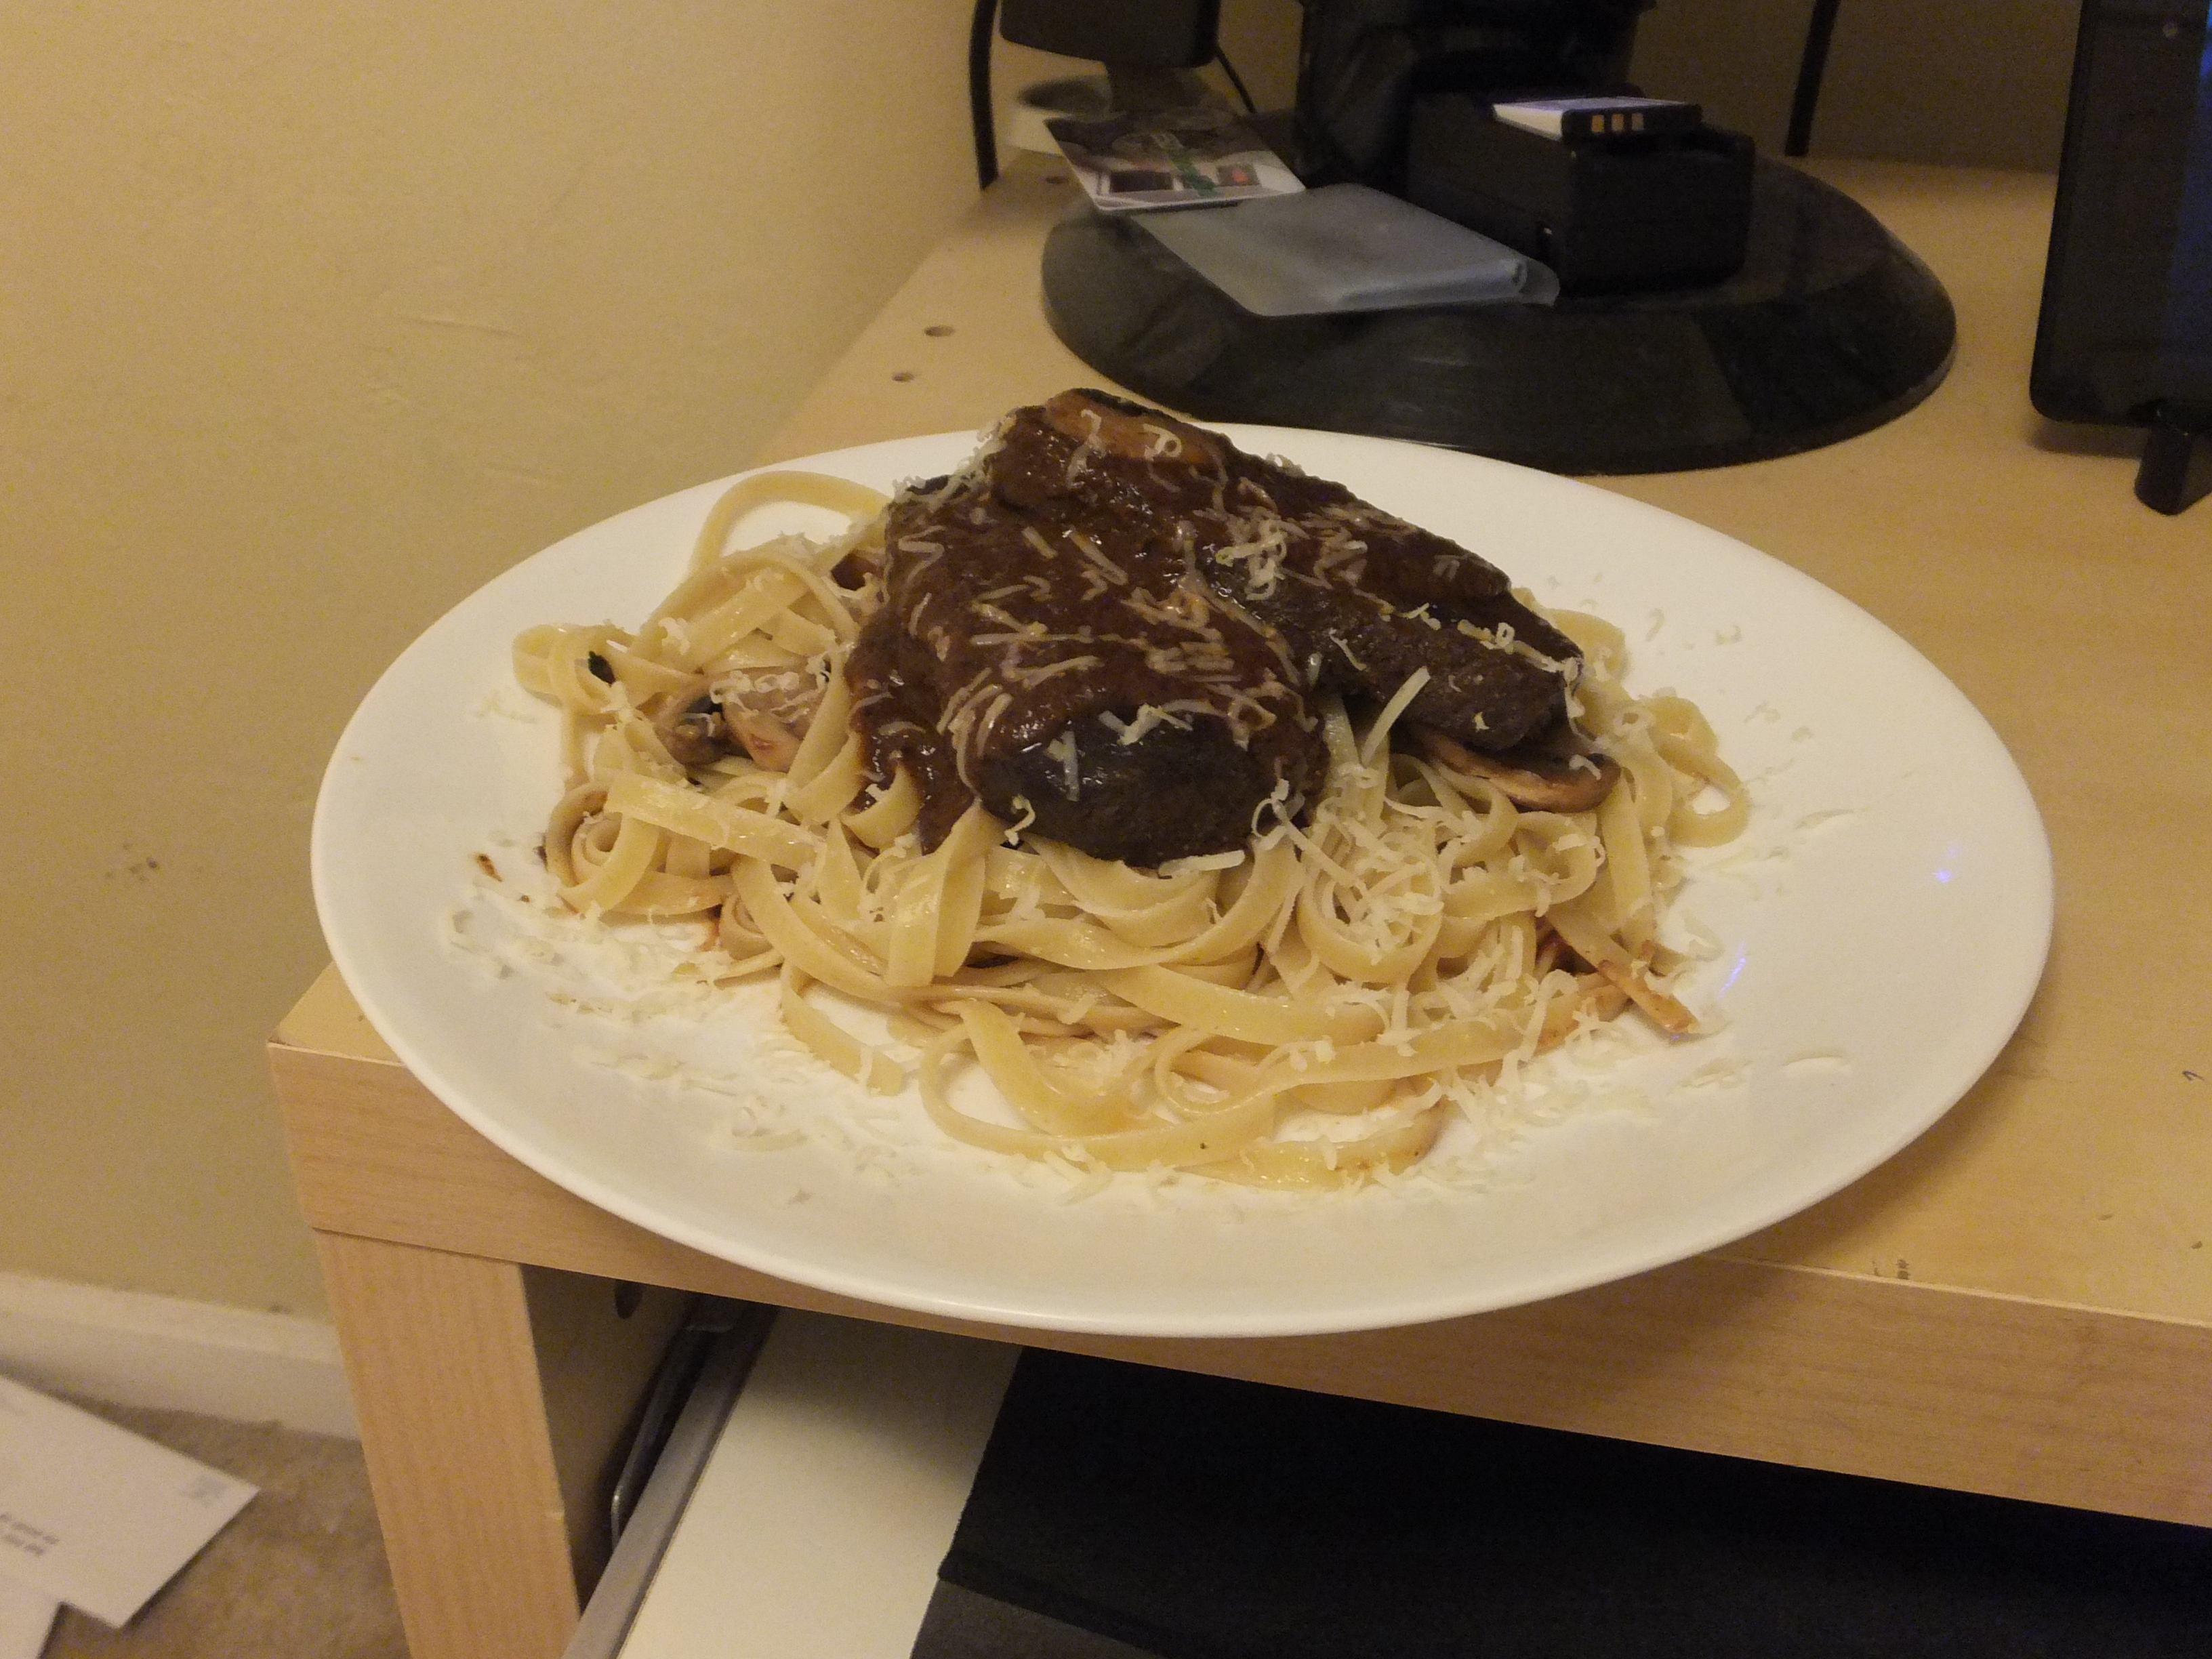
\includegraphics[width=\linewidth,trim=400px 400px 200px 500px, clip=true]{beef_wine_pasta-01.jpeg}
    \end{image}
  \end{images}

  \begin{steps}
  \item Dry and season the beef, allow it to come to room temperature.
  \item Add the butter and olive oil to a pan, get very hot.
  \item Sear the beef in the pan until rare.
  \item Add wine to the pan, deglaze.
  \item Add the tomatoes to the pan.
  \item Simmer for one hour.
  \item Cook some pasta, serve with the beef and sauce.
  \end{steps}

  \begin{notes}
  \item I really should have had a whole onion and canned diced
    tomatoes, but I'm a bum.  To compensate for the lack of onions, I
    tossed some mushrooms in a pan (see \bref{mushrooms_butter}) and
    stirred them into the pasta.  It didn't make a difference.
  \item Thicker pasta would be better, but I never bother with it.
  \item There should be garlic and herbs in this, in addition to the
    onion mentioned earlier.  I actually put in garlic powder and
    oregano, but there should probably have been more stuff in there.
  \item The 8oz of meat probably would have sufficied for 4 of me, it
    would have just required some extra sauce -- even with only 10oz
    of noodles it was pretty dry.
  \end{notes}
\end{recipe}
\end{document}
